% Animation of the two-track inference (Algorithm 2) on the paper's figure.
%
% The picture is the paper's TikZ code, unchanged, with each element wrapped in \only<1,k->{...}:
% it is shown faintly at overlay 1 (overview) and appears for good at overlay k.  Drawn on top of it
% (animation_style.tex): red frames for the observation being processed, red bars under the data a step
% uses, white veils over what is not used, a light band behind the panel being built, and the caption bar.
% Each overlay is one frame; build_animation.py sets how long each frame is shown.
%
%   overlay  1       overview: the whole figure, faint
%   overlays 2-14    Step 1, panel (a): exploration, the two tracks, conditional independence
%   overlays 15-25   Step 2, panel (b): preliminary fit, predictable refit, truncation
%   overlays 26-41   Step 3, panel (c): calibration along the other track, both directions
%   overlays 42-44   cross-fitting: the role of each track and of the exploration record
%   overlays 45-46   Step 4: aggregation; the complete figure
\documentclass[11pt]{beamer}
\usefonttheme{serif}
\geometry{paperwidth=17.0cm,paperheight=13.4cm}
\setbeamertemplate{navigation symbols}{}
\setbeamersize{text margin left=0pt,text margin right=0pt}
\usepackage{amsmath,amssymb}
\usepackage{tikz}
\usetikzlibrary{arrows.meta,calc,positioning,decorations.pathreplacing}
\definecolor{twotrackblue}{HTML}{2F5D8A}
\definecolor{twotrackorange}{HTML}{B66A28}
\definecolor{twotrackgray}{HTML}{4B525A}
% Shared by both animations (two_track_animation.tex, greedy_flow_animation.tex):
% the highlight color, the helpers drawn on top of a figure, and the caption bar.
\definecolor{nowred}{HTML}{C62828}
\definecolor{chipgray}{HTML}{4B525A}
\definecolor{chipteal}{HTML}{267A78}
\pgfdeclarelayer{background}
\pgfsetlayers{background,main}
\tikzset{
  now/.style={draw=nowred,line width=1.3pt,rounded corners=1.5pt},
  usedbar/.style={draw=nowred!60,line width=2pt},
  veil/.style={fill=white,opacity=0.65},
  rednote/.style={text=nowred,font=\scriptsize}
}

% red frame around a node (#1), around its top or bottom half, around a group of nodes (#1 to #2)
\newcommand{\frameall}[1]{\draw[now] ([shift={(-1.2pt,-1.2pt)}]#1.south west) rectangle ([shift={(1.2pt,1.2pt)}]#1.north east);}
\newcommand{\frametop}[1]{\draw[now] ([shift={(-1.2pt,0pt)}]#1.west) rectangle ([shift={(1.2pt,1.2pt)}]#1.north east);}
\newcommand{\framebottom}[1]{\draw[now] ([shift={(-1.2pt,-1.2pt)}]#1.south west) rectangle ([shift={(1.2pt,0pt)}]#1.east);}
\newcommand{\framegroup}[2]{\draw[now] ([shift={(-2.5pt,-2.5pt)}]#1.south west) rectangle ([shift={(2.5pt,2.5pt)}]#2.north east);}
% red frame around a card of the Algorithm 1 figure (larger rounded corners)
\newcommand{\framecard}[1]{\draw[draw=nowred,line width=1.4pt,rounded corners=3pt]
  ([shift={(-2pt,-2pt)}]#1.south west) rectangle ([shift={(2pt,2pt)}]#1.north east);}
% white veil over a node: the part not used at that moment
\newcommand{\veilnode}[1]{\fill[veil] ([shift={(-2pt,-2pt)}]#1.south west) rectangle ([shift={(2pt,2pt)}]#1.north east);}
% red bar under a node: data used by the step in red
\newcommand{\usedbar}[1]{\draw[usedbar] ([shift={(1pt,-3pt)}]#1.south west) -- ([shift={(-1pt,-3pt)}]#1.south east);}
% light band behind the panel being built, from height #1 to height #2
\newcommand{\panelband}[2]{\begin{pgfonlayer}{background}
  \fill[black!3,rounded corners=4pt] (-0.12,#1) rectangle (16.12,#2);\end{pgfonlayer}}

% caption bar under the figure: #1 chip color, #2 chip text, #3 caption (two lines at most)
\newcommand{\captionbar}[3]{%
  \begin{tikzpicture}
    \path[use as bounding box] (0,0) rectangle (16.2,1.45);
    \fill[black!4,rounded corners=3pt] (0,0) rectangle (16.2,1.45);
    \node[fill=#1,text=white,font=\footnotesize\bfseries,rounded corners=2pt,
      minimum width=1.6cm,minimum height=.56cm,inner sep=2pt] at (1.0,.725) {#2};
    \node[anchor=west,text width=13.9cm,align=left,font=\small,text=black!85] at (2.0,.725) {#3};
  \end{tikzpicture}}


\begin{document}
\begin{frame}[plain,t]
\vspace*{2mm}
\centering
\begin{tikzpicture}[
  x=1cm,
  y=1cm,
  font=\scriptsize,
  line cap=round,
  line join=round,
  sample/.style={
    draw=twotrackgray!68,
    fill=white,
    rounded corners=0.8pt,
    minimum width=0.58cm,
    minimum height=0.50cm,
    inner sep=0pt,
    align=center,
    line width=0.55pt
  },
  pilotcell/.style={sample,fill=black!4},
  trackonecell/.style={sample,draw=twotrackblue,
    fill=twotrackblue!10},
  tracktwocell/.style={sample,draw=twotrackorange,
    fill=twotrackorange!11},
  evalonecell/.style={trackonecell,minimum height=0.70cm},
  evaltwocell/.style={tracktwocell,minimum height=0.70cm},
  trackonechip/.style={
    draw=twotrackblue,
    fill=twotrackblue!7,
    rounded corners=2pt,
    line width=0.65pt,
    align=center,
    inner xsep=4pt,
    inner ysep=3pt
  },
  tracktwochip/.style={
    draw=twotrackorange,
    fill=twotrackorange!8,
    rounded corners=2pt,
    line width=0.65pt,
    align=center,
    inner xsep=4pt,
    inner ysep=3pt
  },
  neutralchip/.style={
    draw=twotrackgray!72,
    fill=black!2,
    rounded corners=2pt,
    line width=0.60pt,
    align=center,
    inner xsep=4pt,
    inner ysep=3pt
  },
  outputchip/.style={
    draw=twotrackgray!88,
    fill=black!4,
    rounded corners=2.5pt,
    line width=0.70pt,
    align=center,
    inner xsep=5pt,
    inner ysep=4pt
  },
  flow/.style={
    -{Latex[length=1.75mm,width=1.05mm]},
    draw=twotrackgray!88,
    line width=0.65pt
  },
  mergeflow/.style={
    flow,
    preaction={draw=white,line width=2.2pt,-}
  },
  braceabove/.style={
    decorate,
    decoration={brace,amplitude=3pt},
    draw=twotrackgray!82,
    line width=0.55pt
  },
  bracebelow/.style={
    decorate,
    decoration={brace,amplitude=3pt,mirror},
    draw=twotrackgray!82,
    line width=0.55pt
  },
  sectionrule/.style={draw=black!16,line width=0.45pt}
]
\useasboundingbox (-0.15,-0.42) rectangle (16.15,10.62);

% light band behind the panel being built
\only<2-14>{\panelband{8.42}{10.58}}
\only<15-25>{\panelband{3.22}{8.32}}
\only<26-41,45>{\panelband{-0.38}{3.22}}

% =====================================================================================
% (a) Chronological collection.
% =====================================================================================
\only<1,2->{
  \node[anchor=west,font=\small\bfseries,text=twotrackgray]
    (titlea) at (0,10.28) {(a) Explore and collect};
  \draw[sectionrule] ([xshift=0.22cm]titlea.east) -- (16.0,10.28);
  \draw[-{Latex[length=1.55mm,width=0.95mm]},draw=black!35,
    line width=0.50pt] (0.28,9.34) -- (9.62,9.34)
    node[right=2pt,text=twotrackgray] {\(t\)};
}
\only<1,2->{\node[pilotcell] (sone) at (0.60,9.34) {\(\scriptscriptstyle 1\)};}
\only<1,3->{\node[pilotcell] (stwo) at (1.24,9.34) {\(\scriptscriptstyle 2\)};}
\only<1,4->{\node[pilotcell] (sdots) at (1.88,9.34) {\(\scriptscriptstyle\cdots\)};}
\only<1,5->{\node[pilotcell] (stau) at (2.52,9.34) {\(\scriptscriptstyle \tau\)};}

\only<1,6->{
  \draw[black!18,line width=0.55pt] (3.05,8.90) -- (3.05,9.78);
  \node[trackonecell,minimum width=0.72cm] (d11) at (3.57,9.34)
    {\(\scriptscriptstyle O_1^{(1)}\)};
}
\only<1,7->{\node[tracktwocell,minimum width=0.72cm] (d12) at (4.36,9.34)
    {\(\scriptscriptstyle O_1^{(2)}\)};}
\only<1,8->{\node[trackonecell,minimum width=0.72cm] (d21) at (5.15,9.34)
    {\(\scriptscriptstyle O_2^{(1)}\)};}
\only<1,9->{\node[tracktwocell,minimum width=0.72cm] (d22) at (5.94,9.34)
    {\(\scriptscriptstyle O_2^{(2)}\)};}
\only<1,10->{\node[sample,minimum width=0.72cm] (ddots) at (6.73,9.34)
    {\(\scriptscriptstyle\cdots\)};}
\only<1,11->{\node[trackonecell,minimum width=0.88cm] (dn1) at (7.64,9.34)
    {\(\scriptscriptstyle O_{n_{\rm tr}}^{(1)}\)};}
\only<1,12->{\node[tracktwocell,minimum width=0.88cm] (dn2) at (8.59,9.34)
    {\(\scriptscriptstyle O_{n_{\rm tr}}^{(2)}\)};}

\only<1,13->{
  \draw[bracebelow]
    ([yshift=-2pt]sone.south west) -- ([yshift=-2pt]stau.south east)
    node[midway,below=4pt] {\(\mathcal S_o\)};
  \draw[bracebelow]
    ([yshift=-2pt]d11.south west) -- ([yshift=-2pt]dn2.south east)
    node[midway,below=4pt]
    {\(\mathcal D^{(1)},\mathcal D^{(2)}\)};
}
\only<1,14->{
  \draw[sectionrule] (10.20,8.73) -- (10.20,9.96);
  \node[anchor=west] at (10.62,9.70)
    {\(O_t^{(j)}=(\Xi_t^{(j)},a_t^{(j)},y_t^{(j)})\)};
  \node[anchor=west] at (10.62,9.05)
    {\(\sigma(\mathcal D^{(1)})\perp\!\!\!\perp
      \sigma(\mathcal D^{(2)})\mid\sigma(\mathcal S_o)\)};
}

% =====================================================================================
% (b) Sample segments and track-specific preliminary estimators.
% =====================================================================================
\only<1,15->{
  \node[anchor=west,font=\small\bfseries,text=twotrackgray]
    (titleb) at (0,8.02) {(b) Estimate and refit};
  \draw[sectionrule] ([xshift=0.22cm]titleb.east) -- (16.0,8.02);

  % Track 1 cells.
  \node[pilotcell] (p11) at (0.54,6.55) {\(\scriptscriptstyle 1\)};
  \node[pilotcell] (p12) at (1.18,6.55) {\(\scriptscriptstyle 2\)};
  \node[pilotcell] (p1d) at (1.82,6.55) {\(\scriptscriptstyle\cdots\)};
  \node[pilotcell] (p1t) at (2.46,6.55) {\(\scriptscriptstyle \tau\)};
  \node at (2.88,6.55) {\(+\)};
  \node[trackonecell] (x111) at (3.30,6.55) {\(\scriptscriptstyle O_1^{(1)}\)};
  \node[trackonecell] (x112) at (3.94,6.55) {\(\scriptscriptstyle O_2^{(1)}\)};
  \node[trackonecell] (x11d) at (4.58,6.55) {\(\scriptscriptstyle\cdots\)};
  \node[trackonecell,minimum width=0.72cm] (x11n) at (5.27,6.55)
    {\(\scriptscriptstyle O_{n_0}^{(1)}\)};
  \node[trackonecell,minimum width=0.86cm] (x12a) at (6.12,6.55)
    {\(\scriptscriptstyle O_{n_0+1}^{(1)}\)};
  \node[trackonecell,minimum width=0.86cm] (x12b) at (7.04,6.55)
    {\(\scriptscriptstyle O_{n_0+2}^{(1)}\)};
  \node[trackonecell] (x12d) at (7.78,6.55) {\(\scriptscriptstyle\cdots\)};
  \node[trackonecell,minimum width=0.78cm] (x12n) at (8.50,6.55)
    {\(\scriptscriptstyle O_{n_{\rm tr}}^{(1)}\)};
}
\only<1,16->{
  \draw[braceabove]
    ([yshift=2pt]p11.north west) -- ([yshift=2pt]x11n.north east)
    node[midway,above=4pt,trackonechip] (preone)
    {\(\bigl(\mathcal S_o,\mathcal D_{1:n_0}^{(1)}\bigr)
      \mapsto(\breve\theta^{(1)},\breve P_1,\breve Q_1)\)};
}
\only<1,21->{
  \draw[bracebelow]
    ([yshift=-2pt]x12a.south west) -- ([yshift=-2pt]x12n.south east)
    node[midway,below=4pt,trackonechip] (refone)
    {\(\mathcal D_{n_0+1:n_{\rm tr}}^{(1)}\)};
}
\only<1,22->{
  \node[trackonechip,text width=3.72cm] (nuisone) at (13.42,6.55)
    {\(\displaystyle
      \check\theta^{(1)}
      \xrightarrow{\text{truncate}}
      (\hat\theta^{(1)},\hat P_1)\)};
  \draw[mergeflow] (preone.east) to[out=2,in=158] (nuisone.west);
  \draw[mergeflow] (refone.east) to[out=-2,in=202] (nuisone.west);
}

\only<1,23->{
  % Track 2 cells.
  \node[pilotcell] (p21) at (0.54,4.30) {\(\scriptscriptstyle 1\)};
  \node[pilotcell] (p22) at (1.18,4.30) {\(\scriptscriptstyle 2\)};
  \node[pilotcell] (p2d) at (1.82,4.30) {\(\scriptscriptstyle\cdots\)};
  \node[pilotcell] (p2t) at (2.46,4.30) {\(\scriptscriptstyle \tau\)};
  \node at (2.88,4.30) {\(+\)};
  \node[tracktwocell] (x211) at (3.30,4.30) {\(\scriptscriptstyle O_1^{(2)}\)};
  \node[tracktwocell] (x212) at (3.94,4.30) {\(\scriptscriptstyle O_2^{(2)}\)};
  \node[tracktwocell] (x21d) at (4.58,4.30) {\(\scriptscriptstyle\cdots\)};
  \node[tracktwocell,minimum width=0.72cm] (x21n) at (5.27,4.30)
    {\(\scriptscriptstyle O_{n_0}^{(2)}\)};
  \node[tracktwocell,minimum width=0.86cm] (x22a) at (6.12,4.30)
    {\(\scriptscriptstyle O_{n_0+1}^{(2)}\)};
  \node[tracktwocell,minimum width=0.86cm] (x22b) at (7.04,4.30)
    {\(\scriptscriptstyle O_{n_0+2}^{(2)}\)};
  \node[tracktwocell] (x22d) at (7.78,4.30) {\(\scriptscriptstyle\cdots\)};
  \node[tracktwocell,minimum width=0.78cm] (x22n) at (8.50,4.30)
    {\(\scriptscriptstyle O_{n_{\rm tr}}^{(2)}\)};

  \draw[braceabove]
    ([yshift=2pt]p21.north west) -- ([yshift=2pt]x21n.north east)
    node[midway,above=4pt,tracktwochip] (pretwo)
    {\(\bigl(\mathcal S_o,\mathcal D_{1:n_0}^{(2)}\bigr)
      \mapsto(\breve\theta^{(2)},\breve P_2,\breve Q_2)\)};
}
\only<1,24->{
  \draw[bracebelow]
    ([yshift=-2pt]x22a.south west) -- ([yshift=-2pt]x22n.south east)
    node[midway,below=4pt,tracktwochip] (reftwo)
    {\(\mathcal D_{n_0+1:n_{\rm tr}}^{(2)}\)};
}
\only<1,25->{
  \node[tracktwochip,text width=3.72cm] (nuistwo) at (13.42,4.30)
    {\(\displaystyle
      \check\theta^{(2)}
      \xrightarrow{\text{truncate}}
      (\hat\theta^{(2)},\hat P_2)\)};
  \draw[mergeflow] (pretwo.east) to[out=2,in=158] (nuistwo.west);
  \draw[mergeflow] (reftwo.east) to[out=-2,in=202] (nuistwo.west);
}

% =====================================================================================
% (c) Opposite-track calibration and aggregation.
% =====================================================================================
\only<1,26->{
  \node[anchor=west,font=\small\bfseries,text=twotrackgray]
    (titlec) at (0,3.02) {(c) Calibrate and aggregate};
  \draw[sectionrule] ([xshift=0.22cm]titlec.east) -- (16.0,3.02);

  \node[trackonechip,text width=2.25cm] (etaone) at (1.38,2.14)
    {\((\hat\theta^{(1)},\hat P_1,A)\)};
  \node[evaltwocell] (e21) at (3.47,2.14) {};
  \node[evaltwocell] (e22) at (4.11,2.14) {};
  \node[evaltwocell] (e2d) at (4.75,2.14) {};
  \node[evaltwocell,minimum width=0.76cm] (e2n) at (5.46,2.14) {};
  \draw[twotrackorange!52,line width=0.42pt]
    (e21.west) -- (e21.east) (e22.west) -- (e22.east)
    (e2d.west) -- (e2d.east) (e2n.west) -- (e2n.east);
  \node at ([yshift=0.17cm]e21.center) {\(\scriptscriptstyle z_1^{(2)}\)};
  \node at ([yshift=-0.17cm]e21.center) {\(\scriptscriptstyle y_1^{(2)}\)};
  \node at ([yshift=0.17cm]e22.center) {\(\scriptscriptstyle z_2^{(2)}\)};
  \node at ([yshift=-0.17cm]e22.center) {\(\scriptscriptstyle y_2^{(2)}\)};
  \node at ([yshift=0.17cm]e2d.center) {\(\scriptscriptstyle\cdots\)};
  \node at ([yshift=-0.17cm]e2d.center) {\(\scriptscriptstyle\cdots\)};
  \node at ([yshift=0.17cm]e2n.center)
    {\(\scriptscriptstyle z_{n_{\rm tr}}^{(2)}\)};
  \node at ([yshift=-0.17cm]e2n.center)
    {\(\scriptscriptstyle y_{n_{\rm tr}}^{(2)}\)};
  \node[neutralchip,text width=2.18cm] (weightone) at (7.45,2.14)
    {\(\{(\omega_{1,t},\rho_{1,t})\}_{t=1}^{n_{\rm tr}}\)};
  \draw[mergeflow] (etaone.north) -- (1.38,2.77) -- (7.45,2.77) -- (weightone.north);
  \draw[flow] ([yshift=0.17cm]e2n.east) -- ([yshift=0.17cm]weightone.west);
}
\only<1,35->{
  \node[neutralchip,text width=1.86cm] (foldone) at (10.45,2.14)
    {\((\hat\mu^{(1)},\hat V^{(1)})\)};
  \draw[flow] (weightone.east) -- node[below=2pt,fill=white,inner sep=1pt]
    {\(y_{1:n_{\rm tr}}^{(2)}\)} (foldone.west);
}

\only<1,36->{
  \node[tracktwochip,text width=2.25cm] (etatwo) at (1.38,0.78)
    {\((\hat\theta^{(2)},\hat P_2,A)\)};
  \node[evalonecell] (e11) at (3.47,0.78) {};
  \node[evalonecell] (e12) at (4.11,0.78) {};
  \node[evalonecell] (e1d) at (4.75,0.78) {};
  \node[evalonecell,minimum width=0.76cm] (e1n) at (5.46,0.78) {};
  \draw[twotrackblue!52,line width=0.42pt]
    (e11.west) -- (e11.east) (e12.west) -- (e12.east)
    (e1d.west) -- (e1d.east) (e1n.west) -- (e1n.east);
  \node at ([yshift=0.17cm]e11.center) {\(\scriptscriptstyle z_1^{(1)}\)};
  \node at ([yshift=-0.17cm]e11.center) {\(\scriptscriptstyle y_1^{(1)}\)};
  \node at ([yshift=0.17cm]e12.center) {\(\scriptscriptstyle z_2^{(1)}\)};
  \node at ([yshift=-0.17cm]e12.center) {\(\scriptscriptstyle y_2^{(1)}\)};
  \node at ([yshift=0.17cm]e1d.center) {\(\scriptscriptstyle\cdots\)};
  \node at ([yshift=-0.17cm]e1d.center) {\(\scriptscriptstyle\cdots\)};
  \node at ([yshift=0.17cm]e1n.center)
    {\(\scriptscriptstyle z_{n_{\rm tr}}^{(1)}\)};
  \node at ([yshift=-0.17cm]e1n.center)
    {\(\scriptscriptstyle y_{n_{\rm tr}}^{(1)}\)};
  \node[neutralchip,text width=2.18cm] (weighttwo) at (7.45,0.78)
    {\(\{(\omega_{2,t},\rho_{2,t})\}_{t=1}^{n_{\rm tr}}\)};
  \draw[mergeflow] (etatwo.south) -- (1.38,-.05) -- (7.45,-.05) -- (weighttwo.south);
  \draw[flow] ([yshift=0.17cm]e1n.east) -- ([yshift=0.17cm]weighttwo.west);
}
\only<1,41->{
  \node[neutralchip,text width=1.86cm] (foldtwo) at (10.45,0.78)
    {\((\hat\mu^{(2)},\hat V^{(2)})\)};
  \draw[flow] (weighttwo.east) -- node[below=2pt,fill=white,inner sep=1pt]
    {\(y_{1:n_{\rm tr}}^{(1)}\)} (foldtwo.west);
}

\only<1,45->{
  \draw[decorate,decoration={brace,amplitude=4pt,mirror},
    draw=twotrackgray!88,line width=0.65pt]
    (11.72,0.43) -- (11.72,2.49);
  \node[outputchip,text width=3.36cm,minimum height=1.20cm]
    (aggregate) at (14.05,1.46) {};
  \node at (14.05,1.70)
    {\(\displaystyle\hat\mu=\tfrac12(\hat\mu^{(1)}+\hat\mu^{(2)})\)};
  \node at (14.05,1.22)
    {\(\displaystyle
      \hat V_N=\tfrac12
      \bigl\{\textstyle\sum_{\ell=1}^{2}(\hat V^{(\ell)})^2\bigr\}^{1/2}\)};
  \draw[flow] (11.96,1.46) -- (aggregate.west);
}

% =====================================================================================
% Highlights (drawn on top of the figure)
% =====================================================================================
% overview: the whole figure, faint
\only<1>{\fill[white,opacity=0.72] (-0.15,-0.42) rectangle (16.15,10.62);}

% Step 1: the observation collected (red frame) and the data its track may use (red bars)
\only<6>{\frameall{d11}\foreach \c in {sone,stwo,sdots,stau} {\usedbar{\c}}}
\only<7>{\frameall{d12}\veilnode{d11}\foreach \c in {sone,stwo,sdots,stau} {\usedbar{\c}}}
\only<8>{\frameall{d21}\veilnode{d12}\foreach \c in {sone,stwo,sdots,stau,d11} {\usedbar{\c}}}
\only<9>{\frameall{d22}\veilnode{d11}\veilnode{d21}\foreach \c in {sone,stwo,sdots,stau,d12} {\usedbar{\c}}}
\only<11>{\frameall{dn1}\veilnode{d12}\veilnode{d22}\foreach \c in {sone,stwo,sdots,stau,d11,d21} {\usedbar{\c}}}
\only<12>{\frameall{dn2}\veilnode{d11}\veilnode{d21}\veilnode{dn1}\foreach \c in {sone,stwo,sdots,stau,d12,d22} {\usedbar{\c}}}

% Step 2: preliminary fit, then the predictable refit one observation at a time
\only<16>{\foreach \c in {p11,p12,p1d,p1t,x111,x112,x11d,x11n} {\usedbar{\c}}}
\only<17>{\frameall{x12a}\node[rednote,below=3pt] at (x12a.south) {\(w^{\rm ref}_{1,t}\) before \(y^{(1)}_t\)};}
\only<18>{\frameall{x12b}\node[rednote,below=3pt] at (x12b.south) {\(w^{\rm ref}_{1,t}\) before \(y^{(1)}_t\)};}
\only<19>{\frameall{x12d}}
\only<20>{\frameall{x12n}\node[rednote,below=3pt] at (x12n.south) {\(w^{\rm ref}_{1,t}\) before \(y^{(1)}_t\)};}
\only<22>{\frameall{nuisone}}
\only<23>{\foreach \c in {p21,p22,p2d,p2t,x211,x212,x21d,x21n} {\usedbar{\c}}}
\only<25>{\frameall{nuistwo}}

% Step 3: on the other track, the design z_t first (weight), then the response y_t
\only<26>{\frameall{etaone}}
\only<27,29,31,33>{\node[rednote,below=1pt] at (weightone.south) {\(\omega_{1,t}\) from \(z^{(2)}_t\) and earlier rounds};}
\only<28,30,32,34>{\node[rednote,below=1pt] at (weightone.south) {then \(y^{(2)}_t\) enters the correction};}
\only<27>{\frametop{e21}\frameall{weightone}}
\only<28>{\framebottom{e21}}
\only<29>{\frametop{e22}\frameall{weightone}}
\only<30>{\framebottom{e22}}
\only<31>{\frametop{e2d}\frameall{weightone}}
\only<32>{\framebottom{e2d}}
\only<33>{\frametop{e2n}\frameall{weightone}}
\only<34>{\framebottom{e2n}}
\only<35>{\frameall{foldone}}
\only<36>{\frameall{etatwo}}
\only<37>{\frametop{e11}\frameall{weighttwo}}
\only<38>{\framebottom{e11}}
\only<39>{\frametop{e1n}\frameall{weighttwo}}
\only<40>{\framebottom{e1n}}
\only<41>{\frameall{foldtwo}}

% cross-fitting: what each track and the exploration record are used for
\only<42>{\framegroup{x111}{x12n}\frameall{nuisone}\framegroup{e11}{e1n}\frameall{foldtwo}
  \foreach \c in {x211,x212,x21d,x21n,x22a,x22b,x22d,x22n,nuistwo,e21,e22,e2d,e2n,foldone} {\veilnode{\c}}
  \node[rednote,anchor=west] at ([xshift=4pt]x12n.east) {fit};
  \node[rednote,anchor=west] at ([xshift=4pt,yshift=-9pt]foldtwo.east) {correction};}
\only<43>{\framegroup{x211}{x22n}\frameall{nuistwo}\framegroup{e21}{e2n}\frameall{foldone}
  \foreach \c in {x111,x112,x11d,x11n,x12a,x12b,x12d,x12n,nuisone,e11,e12,e1d,e1n,foldtwo} {\veilnode{\c}}
  \node[rednote,anchor=west] at ([xshift=4pt]x22n.east) {fit};
  \node[rednote,anchor=west] at ([xshift=4pt,yshift=-9pt]foldone.east) {correction};}
\only<44>{\framegroup{sone}{stau}\framegroup{p11}{p1t}\framegroup{p21}{p2t}
  \framegroup{etaone}{foldone}\framegroup{etatwo}{foldtwo}
  \node[rednote,anchor=west] at ([xshift=4pt]foldone.east) {no \(\mathcal S_o\)};
  \node[rednote,anchor=west] at ([xshift=4pt]foldtwo.east) {no \(\mathcal S_o\)};}

% Step 4
\only<45>{\frameall{aggregate}}
\end{tikzpicture}

\vspace{2mm}
% =====================================================================================
% Caption bar (one per overlay)
% =====================================================================================
\only<1>{\captionbar{chipgray}{Goal}{A confidence interval for a prespecified linear functional
  \(\mu^*=\langle A,\theta^*\rangle\), from data collected adaptively by greedy selection.}}%
\only<2-5>{\captionbar{chipgray}{Step 1}{Shared exploration: \(\tau\) uniformly chosen rounds give the
  record \(\mathcal S_o\) and the pilot estimate \(\widetilde\theta\).}}%
\only<6-12>{\captionbar{chipgray}{Step 1}{The rounds alternate between two tracks. Track \(j\) selects
  \(a_t^{(j)}=\arg\max_{a}\langle z_{t,a}^{(j)},\hat\theta_{\tau+t-1}^{(j)}\rangle\) from \(\mathcal S_o\)
  and its own earlier observations only (red bars).}}%
\only<13-14>{\captionbar{chipgray}{Step 1}{So the two records are independent given \(\mathcal S_o\):
  one track's fit can be held fixed while the other corrects it.}}%
\only<15-16>{\captionbar{chipgray}{Step 2}{Each track separately, with \(\mathcal S_o\) in front: fit on
  \(\mathcal S_o\) and the first \(n_0\) observations and keep rank \(r_0\), giving \(\breve\theta^{(1)}\),
  its tangent-space projector \(\breve P_1\) and basis \(\breve Q_1\).}}%
\only<17-21>{\captionbar{chipgray}{Step 2}{Refit on the rest, one observation at a time, each weight
  fixed before \(y^{(1)}_t\) is used:
  \(\check\theta^{(1)}=\breve\theta^{(1)}+\breve Q_1\sum_{t>n_0}w^{\rm ref}_{1,t}
  \{y^{(1)}_t-\psi'(\langle z^{(1)}_t,\breve\theta^{(1)}\rangle)\}\).}}%
\only<22-25>{\captionbar{chipgray}{Step 2}{Truncating \(\check\theta^{(1)}\) to rank \(r_0\) gives
  \(\hat\theta^{(1)}\) and \(\hat P_1\), the fit that Track 2 will correct. The same on Track 2 gives
  \(\hat\theta^{(2)}\) and \(\hat P_2\).}}%
\only<26-34>{\captionbar{chipgray}{Step 3}{With \((\hat\theta^{(1)},\hat P_1)\) held fixed, Track 2
  corrects \(\langle A,\hat\theta^{(1)}\rangle\) in track order: \(\omega_{1,t}\) uses \(z^{(2)}_t\) and
  earlier observations, not \(y^{(2)}_t\), so the weighted errors are martingale differences given
  \((\mathcal S_o,\mathcal D^{(1)})\).}}%
\only<35>{\captionbar{chipgray}{Step 3}{Fold 1: \(\hat\mu^{(1)}=\langle A,\hat\theta^{(1)}\rangle
  +\sum_{t=1}^{n_{\rm tr}}\{y^{(2)}_t-\psi'(\langle z^{(2)}_t,\hat\theta^{(1)}\rangle)\}\,\omega_{1,t}\),\\
  \((\hat V^{(1)})^2=\sum_{t=1}^{n_{\rm tr}}\{y^{(2)}_t-\psi'(\langle z^{(2)}_t,\hat\theta^{(1)}\rangle)\}^2\omega_{1,t}^2\).}}%
\only<36-41>{\captionbar{chipgray}{Step 3}{Roles exchanged: Track 1 corrects the fit from Track 2,
  giving \(\hat\mu^{(2)}\) and \(\hat V^{(2)}\).}}%
\only<42-44>{\captionbar{chipgray}{Step 3}{Cross-fitting: each track fits once, in (b), and corrects
  the other track's fit once, in (c). The exploration record \(\mathcal S_o\) enters both fits but
  neither correction.}}%
\only<45>{\captionbar{chipgray}{Step 4}{Average the two folds. The interval
  \([\hat\mu-z_{1-\delta/2}\hat V_N,\ \hat\mu+z_{1-\delta/2}\hat V_N]\) has asymptotic coverage
  \(1-\delta\).}}%
\only<46>{\captionbar{chipgray}{Steps 1--4}{Two-track data collection and cross-fitted inference for
  \(\mu^*=\langle A,\theta^*\rangle\).}}%
\end{frame}
\end{document}
